		To better understand the dynamics of \eqref{eq:fullPDE}, first let $G\equiv0$. This removes any interaction between particles and the equation becomes
		\begin{equation}\label{eq:OUFPE}
			\partial_t f_t(x,v) = -v\partial_x f_t(x,v) +\partial_v vf_t(x,v) + \sigma \partial_{vv}f_t(x,v).
		\end{equation}
		This is the Fokker-Planck equation for the following system:
		\begin{equation}\label{eq:2dOU}\begin{cases}
			\dif x_t = v_t\dif t\\
			\dif v_t = -v_t\dif t + \sqrt{2\sigma} \dif W_t. 
		\end{cases}	\end{equation}
		Here, $W_t$ is a standard one-dimensional Wiener process. We recognise this as overdamped Langevin dynamics, and so we can exactly calculate the unique invariant measure. To do so it is necessary to solve $\partial_t \rho_t = 0$, that is, when is the density not changing in time. The evolution in $v$ is described by an Ornstein-Uhlenbeck process so it is known that the unique stationary distribution is Gaussian with mean $1$ and variance $\sigma$. The position $x$ depends only on $v$ with no noise. There is no reason to assume any sort of mean reverting behaviour and expect the density to spread out uniformly on the torus. A guess at the solution would then be $\rho (x,v) = \frac{1}{2\pi}\exp(\frac{-v^2}{2})$, with some normalising constant. Notice that this equation does not depend on $x$. By substitution into the stationary Fokker-Planck equation, this is indeed a solution.
        
        Similarly, when $G\not\equiv 0$ the density $f_t(x,v)$ of \eqref{eq:fullPDE} is the Fokker-Planck equation of the two dimensional SDE,
		    \begin{equation}\label{eq:McKV}\begin{cases}
		    \dif x_t = v_t\dif t\\
		    \dif v_t = \left[G(M(t,x_t))-v_t\right] \dif t + \sqrt{2\sigma} \dif W_t. 
			\end{cases} \qquad  (x_t,v_t) \in \T \times \R
			\end{equation}
		This is a McKean-Vlasov equation as the function $M(t,x_t)$ conceals a dependence on the law of the process. 
        \[
            M(t,x) = \frac{\E\left[ v'_t \phi(x-x'_t)\right]}{\E\left[\phi(x-x'_t)\right]}
        \]
        The pair $(x'_t,v'_t)$ is a random variable equal in distribution to $(x_t,v_t)$. This representation of $M(t,x)$ is the same as the one given previously, however in this setting it is natural to use expectation notation over integrals. To illustrate the necessity of introducing another random variable, albeit one that is equal in law, consider the case when the interaction function is the indicator on the interval $[-b,b]$, $\phi(x) = \mathbbm{1}_{[-b,b]}(x)$. This does not meet the requirements in Section \ref{sec:model}, in particular it is neither strictly positive nor does it have unit integral. 
        \begin{align*}
            M(t,x) &=  \frac{\int_{\T}\int_{\R}f_t(y,w)\phi(x-y)w\dif w \dif y}{\int_{\T}\int_{\R}f_t(y,w)\phi(x-y)\dif w \dif y}\\
            &=  \frac{\int_{\T}\int_{\R}f_t(y,w) \mathbbm{1}_{[-b,b]}w\dif w \dif y}{\int_{\T}\int_{\R}f_t(y,w) \mathbbm{1}_{[-b,b]}\dif w \dif y}\\
            &= \frac{\E\left[ v'_t \mathbbm{1}_{[-b,b]}\right]}{\P(x' \in \left[x-b,x+b\right])}\\
            &= \E\left[ v'_t|x' \in [x-b,x+b] \right]
        \end{align*}
        This calculation also illustrates how $\phi$ describes the interaction or `where to look' while $M$ acts as a average velocity of the points `within range'. The transport term, $\partial_v\left( \left[ v-G(M(t,x))\right]f_t(x,v)\right)$ then acts to change the velocity towards the local average given by $M$. It is in this sense that $G$ is the herding function `herding' the system towards a common velocity.
        
        The McKean-Vlasov representation of the system is also the weak+++not weak limit, mention convergence of empirical measure to solution f +++ limit of an $N$-body particle system described by
        \begin{equation}\label{eq:fullparticle}\begin{cases}
            \dif x^{i,N}_t = v^{i,N}_t\dif t\\
            \dif v^{i,N}_t = -v^{i,N}_t\dif t + G\left(\frac{\frac{1}{N}\sum_{j=1}^N \phi(x_t^{i,N} - x_t^{j,N})v^{j,N}_t  }{\frac{1}{N}\sum_{j=1}^N \phi(x_t^{i,N} - x_t^{j,N})}\right)\dif t + \sqrt{2\sigma} \dif W^i_t 
            \end{cases}, \qquad  i = 1,\dots,N.
        \end{equation}
        This gives another view of the full system \eqref{eq:fullPDE}, and one that is particularly amenable to analysis. It also allows a more intuitive view of the system -- rather than thinking of how a density changes over time, we can think of particles moving around a torus and interacting according to $\phi$.
        
        \subsection{Invariant Measures under Space Homogeneity}\label{sec:hominvmeas}
        Thus far, we have found the invariant measure for only the rather uninteresting case when $G \equiv 0$. To progress further, we must simplify the system. One way to do this is to impose that the density does not depend on the position in space and set $\phi \equiv 1$. The weighted local average velocity $M$ becomes neither local nor weighted. In the particle system, this means that each particle interacts with every other particle, irrespective of the distance between them. Indeed,
        \begin{align*}
            M(t,x) =&  \frac{\int_{\T}\int_{\R}f_t(y,w)\phi(x-y)w\dif w \dif y}{\int_{\T}\int_{\R}f_t(y,w)\phi(x-y)\dif w \dif y}\\
            =&  \frac{\int_{\T}\int_{\R}f_t(y,w)w\dif w \dif y}{\int_{\T}\int_{\R}f_t(y,w)\dif w \dif y}\\
            =& \int_{\T}\int_{\R}f_t(y,w)w\dif w \dif y\\
            :=& \langle w \rangle_{f_t}.
        \end{align*}
        So the weighted local average velocity is just the average of the distribution $f_t(v)$ or equivalently, the average velocity of all particles in the system. The evolution is then described by
        \begin{equation}\label{eq:spacehomPDE}
            \partial_t f_t(v) = \partial_v vf_t(v) - \partial_v G(\langle w \rangle_{f_t})f_t(v) + \sigma \partial_{vv} f_t(v).
        \end{equation}
        The above problem's well-posedness can be shown as follows. Let
        \[
            h_t(v) = f_t(u),\text{ where } u = v + \int_0^t G(\langle w\rangle_{f_t}) \dif s.
        \]
        To find an equation that $h_t(v)$ solves, we use the chain rule.
        \begin{align*}
            \partial_t f_t(u) &= \partial_t f_t(u) +  G(\langle w\rangle_{f_t})\partial_v f_t(u) && \text{as   } \pd{g}{v} = 1, \pd{g}{t} = G((\langle w\rangle_{f_t})\\
            &=\partial_v vf_t(u) - \partial_v G(\langle w \rangle_{f_t})f_t(u) + \sigma \partial_{vv} f_t(u) + G(\langle w\rangle_{f_t})\partial_v f_t(u) &&\text{as  } f_t \text{ solves } \eqref{eq:spacehomPDE}\\
            &=\partial_v vh_t(v) + \sigma \partial_{vv} h_t(v) , \qquad h_0(v) =f_0(v).
        \end{align*}
        So $h_t$ solves the Fokker-Planck equation for the one-dimensional Ornstein-Uhlenbeck process which is well posed. Therefore the solution $f_t(v)$ of \eqref{eq:spacehomPDE} exists and is unique given initial data. To find invariant measures of this evolution, set the transient term to zero and solve the remaining PDE, which can be written in gradient form. First note that if $G\equiv 0$, this system for $f_t$ is the same as that for $h_t$, and so has a unique invariant measure $\mathcal{N}(0,\sigma)$. When the herding function is non-zero, other measures are also stationary as we will now show. For brevity, we omit the dependence on $v$ of $f$ and write $\langle w \rangle_{f_t} = M_1$. The latter is natural as it denotes the first moment of the distribution.
        \begin{align*}
            &\partial_v\left[(-G(M_1) +v) f + \sigma \partial_v f \right] = 0\\
            \implies& (-G(M_1) +v) f + \sigma \partial_v f = C_1
        \end{align*}
        This ODE is solvable and gives 
        \[
            f(v) = C_2\exp\left(\frac{2G(M_1)v - v^2}{2\sigma} \right). 
        \]
        Applying the constraint $\int_\R f(w)\dif w = 1$ gives $C_2 = \exp(-G^2(M_1))/\sqrt{2\pi\sigma}$. This is then a Gaussian distribution with mean $G(M_1)$, and so $M_1 = G(M_1)$. That is, from the definition of space average,
        \begin{align*}
            M_1 :=& \int_\R wf(w) \dif w\\ 
            =& \int_\R \frac{w\exp(-G^2(M_1))}{\sqrt{2\pi\sigma}} \exp\left(\frac{2G(M_1)v - v^2}{2\sigma} \right)\\ 
            =& \int_\R \frac{w}{\sqrt{2\pi\sigma}} \exp\left(\frac{ - (v-G(M_1))^2}{2\sigma} \right)\\
            =& G(M_1)
        \end{align*}
        Using the smoothed version of the herding function from Section \ref{sec:model} gives $G(M_1) = 0, \pm 1$. Substituting this into our expression for $f$ gives three invariant measures:
        \begin{align*}
            \rho_0 &= \frac{1}{\sqrt{2\pi\sigma}}\exp\left(-\frac{v^2}{2\sigma} \right), && \rho_{\pm} = \frac{1}{\sqrt{2\pi\sigma}}\exp\left(-\frac{(v\pm 1)^2}{2\sigma}\right).
        \end{align*}
        These are Gaussian densities with mean $0, \pm 1$ and variance $\sigma$.
        
        We have found three invariant measures for the evolution \eqref{eq:spacehomPDE}, however whether the system will converge to these distributions given initial data remains to be settled. In the space homogeneous case it is possible to close equations on the moments of the distribution. Let $M_n = \int_\R v^n f_t(v) \dif v$ denote the n$^\text{th}$ moment of the distribution $f_t(v)$. Then
        \begin{align*}
            \partial_t M_n(t) &= \int_{\R}v^n \partial_t  f_t(v) \dif v\\
            &= - \int_{\R}v^n \partial_v G(M_1)f_t(v) \dif v + \int_{\R}v^n \partial_v vf_t(v) \dif v + \sigma \int_{\R}v^n \partial_vv f_t(v) \dif v,
        \end{align*}
        as $f_t$ solves the space-homogeneous PDE \eqref{eq:spacehomPDE}. Using integration by parts and simplifying gives, for the first three moments,
        \begin{align}\label{eq:momode}
            \dot{M}_0 &= 0,\notag \\
            \dot{M}_1 &= G(M_1) - M_1,\\
            \dot{M}_2 &= - 2\lbrack M_2 -  M_1G(M_1)  - \sigma\rbrack\notag.
        \end{align}
        The first tells us there is no change in the zeroth moment over time, that is probability is conserved. The equation for the first moment has equilibria at -1, 0 and 1 for the smoothed choice of $G$. Figure \ref{fig:M1phase} shows the phase plane diagram for this ODE. It shows that given any initial data with positive average velocity, the first moment will converge to one. By symmetry, the same is true for negative initial data, the mean will converge towards negative one. It also shows that mean zero is an unstable equilibrium -- a slight perturbation will move the system from random movement to ordered motion.
        \begin{figure}
            \centering
            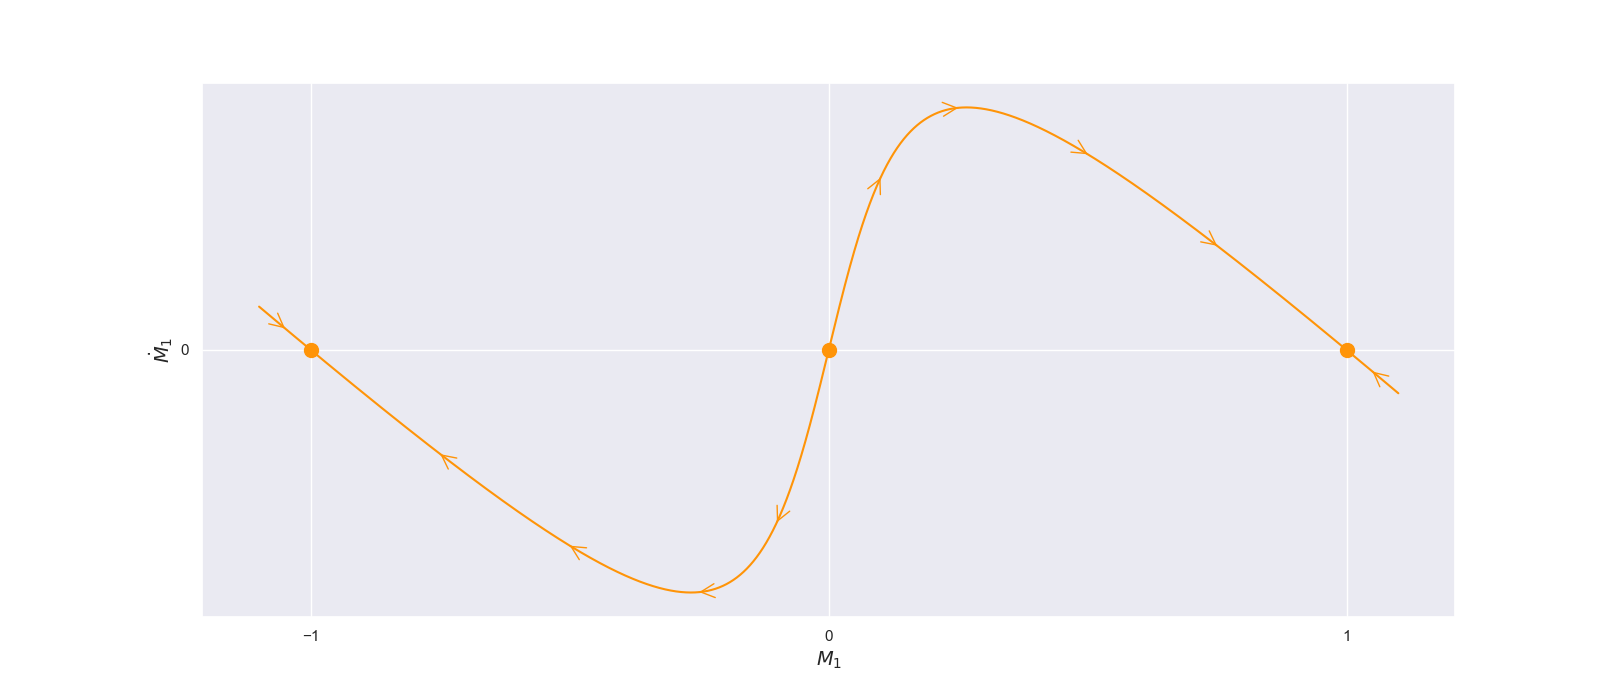
\includegraphics[width=\linewidth]{Figures/M1phase}
            \caption{Phase plane of the first moment ODE with equilibria marked by points assuming a smooth herding function $G$}
            \label{fig:M1phase}
        \end{figure}
        To find the convergence of the variance, we must look at the difference between the second moment and the square of the first.
        \begin{align*}
            \od{}{t}\lbrack M_2 - M_1^2\rbrack &= \dot{M}_2 - 2M_1\dot{M}_1\\
            &= 2\lbrack G(M_1)M_1 - M_2 +\sigma\rbrack - 2M_1\lbrack G(M_1) - M_1\rbrack\\
            &= -2M_2 +2\sigma + 2M_1^2\\
            &= -2\lbrack M_2 - M_1^2 -\sigma\rbrack             
        \end{align*}
        Solving this ODE gives $M_2-M_1^2 = \sigma +(\sigma_0-\sigma)\mathrm{e}^{-2t}$, where $\sigma_0$ is the variance of the initial data $f_0$. Then as $t \to \infty$, it can be seen that the system forgets its initial data and tends towards a distribution with variance $\sigma$.
        
        The equations on the moments have shown that the system indeed converges to a measure with mean $\pm 1$ and variance $\sigma$ however this is not sufficient to conclude that they are Gaussian. To do so requires closing equations on all the cumulants of the distribution. It can be shown that these vanish for all cumulants of order greater than three and so the system indeed converges towards the invariant measures found by solving the space-homogeneous PDE \eqref{eq:spacehomPDE}. This means that irrespective of initial data, we expect all particles to move on average in the same direction with the same velocity -- a phenomenon known as unconditional flocking. The only exception is when the initial data has mean zero. In this case the system will converge to the Gaussian with mean zero, corresponding to disordered motion.
        
        The dynamics of the space-homogeneous system have thus been fully characterised analytically. We will now turn our attention to the particle model in this case.
    \subsubsection{Particle System Dynamics}\label{sec:particledynamics}
        As the particle system approximates the McKean-Vlasov SDE, whose density solves the PDE \eqref{eq:spacehomPDE}, one would expect that it behaves in entirely the same way. This is in fact not the case, as we will now show. Consider the particle system \eqref{eq:fullparticle} in the space-homogeneous case,
        \begin{equation}\label{eq:homparticle}
            \dif v^{i,N}_t = G\left(\frac{1}{N}\sum_{j=1}^N v^{j,N}_t\right)\dif t-v^{i,N}_t \dif t + \sqrt{2\sigma} \dif W^i_t
        \end{equation}
        It has been shown for the kinetic model that the invariant measures have mean zero and $\pm 1$ when we consider a smoothed herding function. Here we will show that the space-homogeneous particle model only admits invariant measures with mean zero for any herding function satisfying the earlier requirements in Section \ref{sec:model}, before finding analytic forms for the functions we will be using. First note that in the case of no interaction, that is $G\equiv 0$, the dynamics are governed by an Ornstein-Uhlenbeck process leading to a unique stationary distribution with mean zero. This is in agreement with the solution to the PDE under no interaction in Section \ref{sec:dynamics}. When $G\not\equiv 0$, the invariant distribution still always has mean zero, unlike what we have seen for the space-homogeneous kinetic model. Given that we wish to find the behaviour of the mean velocity, it would be pertinent to find an equation that it solves. To this end, let $m_t = \frac{1}{N}\sum_{j=1}^N v^{j,N}_t$. Summing the system across $i$ gives an equation for $m_t$:
        \[
            \dif m_t = \lbrack -m_t + G(m_t)\rbrack \dif t +\sqrt{2\sigma}\dif W_t
        \]
        Let $V(x) = \frac{x^2}{2} + \tilde{V}(x)$, where $-\tilde{V}'(x) = G(x)$ so that $-V'(x) = -x + G(x)$. The aim here is to find a function $V$ such that the equation for $m_t$ resembles the Langevin equation. The existence and uniqueness of the invariant measure will then follow from standard theory for the Langevin equation and its associated Fokker-Planck equation. Thus
        \begin{equation}\label{eq:meanSDE}
            \dif m_t = -V'(m_t)\dif t + \sqrt{2\sigma}\dif W_t.
        \end{equation}    
        By definition, $\tilde{V}(x) = - \int_{-\infty}^x G(u) \dif u$. As $G$ is bounded, $\tilde{V}(x)$ grows at most linearly. This means $V(x) \to \infty$ as $|x|\to \infty$, $V$ is a well-defined potential well and $\mathrm{e}^{-V(x)}$ is integrable. Hence \eqref{eq:meanSDE} admits a unique invariant measure, $\rho(x) = \mathcal{Z}^{-1}\mathrm{e}^{-V(x)}$ with $\mathcal{Z}$ a normalising constant.
        
        What can we say about this invariant measure? Recall the only restrictions placed on $G$ in Section \ref{sec:model} were firstly $G$ must be odd, that is $G(u)=-G(-u)$, and secondly,
        \[
            \begin{cases}
            G(u)>u & \text{if } 0<u<1,\\ 
            G(u)<u &  \text{if } u>1.
            \end{cases}
        \]
         
        If $G$ is odd, $\tilde{V}(x)$ is an even function, so $V(x)$ is also an even function. Then the mean of the invariant distribution $\rho$ is
        \[
            \mathbb{E}_{\rho}[m] = \mathcal{Z}^{-1}\int_{\mathbb{R}} m \mathrm{e}^{-V(m)}\dif m = 0,
        \]
        as this is the integral of an odd function. The behaviour of the particle system is then fundamentally different to that of its corresponding kinetic model, despite weakly+++check+++ converging to the McKean-Vlasov SDE \eqref{eq:McKV} whose density solves the PDE \eqref{eq:spacehomPDE}. This is in fact a well-known problem in the area of mean field equations +++cite+++. 
        
    The behaviour of the particle system here is not wholly unexpected -- the change in velocity is inherently random. To see how this affects the invariant measure, first recall the case when $G\equiv 0$, in which the particle system is the Ornstein-Uhlenbeck process and the kinetic model is its corresponding Fokker-Planck equation \eqref{eq:OUFPE}. Here, the particle moves in a potential well with a parabolic shape with a minima at zero. When $G\not\equiv 0$, the particles move within a double-well potential. For the choices of the herding function described here, this well will have minima at -1, 0 and 1\footnote{This is not quite true for any sigmoid $G$ in which $\alpha$ is not large enough.}. Moving deterministically,as the evolution described by the kinetic model is, the particles must settle in one of the two wells leading to a system with mean 1, 0 or -1. Under random movement however, there is a chance that the Wiener process forces the particle to jump over the potential barrier and into the other well. If this happens to enough particles, the remaining particles will also make the jump due to the effect of the herding function. We thus expect, for a finite number of particles, the motion to switch randomly between having average velocity positive one and negative one leading to the invariant measure having mean zero. This switching of mean velocity is known as metastability -- the Gaussian invariant measures for the PDE are only metastable in the particle model. We emphasise again that the dynamics under the kinetic model are fully deterministic and as such no switch of stability is possible.
        
        \begin{figure}
            \centering
        %    \includegraphics[width=0.7\linewidth]{" "}
            \caption{+++Particles in wells. Parabolic (OU) and Double Well showing jump between use draw.io+++}
            \label{fig:particlewells}
        \end{figure}
        
        The method used above to characterise the mean of the distribution gives all that is required to calculate closed forms of the invariant measure. Table \ref{tab:spaceparticleinv} gives expressions for the three herding functions given in Section \ref{sec:model}.
        \begin{table}
        \centering
        \begin{tabular}{|c|c|c|}
            \hline 
            & & \\[-0.5em] 
            & Herding Function & Invariant Measure \\[10pt]
            \hline
            & & \\[-0.5em] 
            Step & $\frac{1+\mathrm{sgn}(u)}{2}$ & +++not correct, not double well or normalised+++ $\exp\left(\frac{|v|}{2}\right)$ \\[10pt]
            \hline 
            & & \\[-0.5em]
            Smooth &$\frac{\arctan(u)}{\arctan(1)}$  & $\frac{1}{(v^2+1)^{\frac{2}{\pi}}} \exp\left( -\frac{v^2}{2}+\frac{4}{\pi}v\mathrm{arctan}(v)\right)$ \\[10pt]
            \hline 
            & & \\[-0.5em]
            Sigmoid & $\frac{2}{1+\mathrm{e}^{-\alpha u}} - 1$ & $ \mathcal{Z}^{-1}(\mathrm{e}^{\alpha v}+1)^{\frac{2}{\alpha}}\exp\left(-\frac{v^2}{2} - v\right)$ \\[10pt]
            \hline 
        \end{tabular}
        \caption[Space-Homogeneous Particle Densities]{Normalised densities for the space-homogeneous particle model \eqref{eq:homparticle} with different herding functions}
        \label{tab:spaceparticleinv}
        \end{table}
    
        \begin{figure}[h!]
            \centering
            %\includegraphics[width=0.7\linewidth]{}
            \caption[Potential Wells]{Potential Wells for the invariant measure of the space-homogeneous particle system for various herding functions}
            \label{fig:spacehomparticlemeasure}
        \end{figure}
        In the space-homogeneous case, the analysis above gives a full picture of the dynamics of both the particle model and the kinetic model. However, the full system \eqref{eq:fullPDE} is much harder to analyse. It can be shown that the invariant measures for \eqref{eq:spacehomPDE} are also invariant, however it cannot be shown that they are the only ones. In particular, it can not be expressed in a gradient form like it could be in the space-homogeneous case. The aim now is to exploit our understanding of the space-homogeneous case to develop robust numerical techniques to learn more about the full system.